\section{Circuitos digitais, expressões booleanas e tabela verdade}
\frame{
	\frametitle{O que vimos até agora?}
	\begin{block}{}
		\begin{itemize}
			\item Circuitos Lógicos.
			\item Expressões booleanas.
			\item Tabela verdade.
		\end{itemize}
	\end{block}
	\centerline{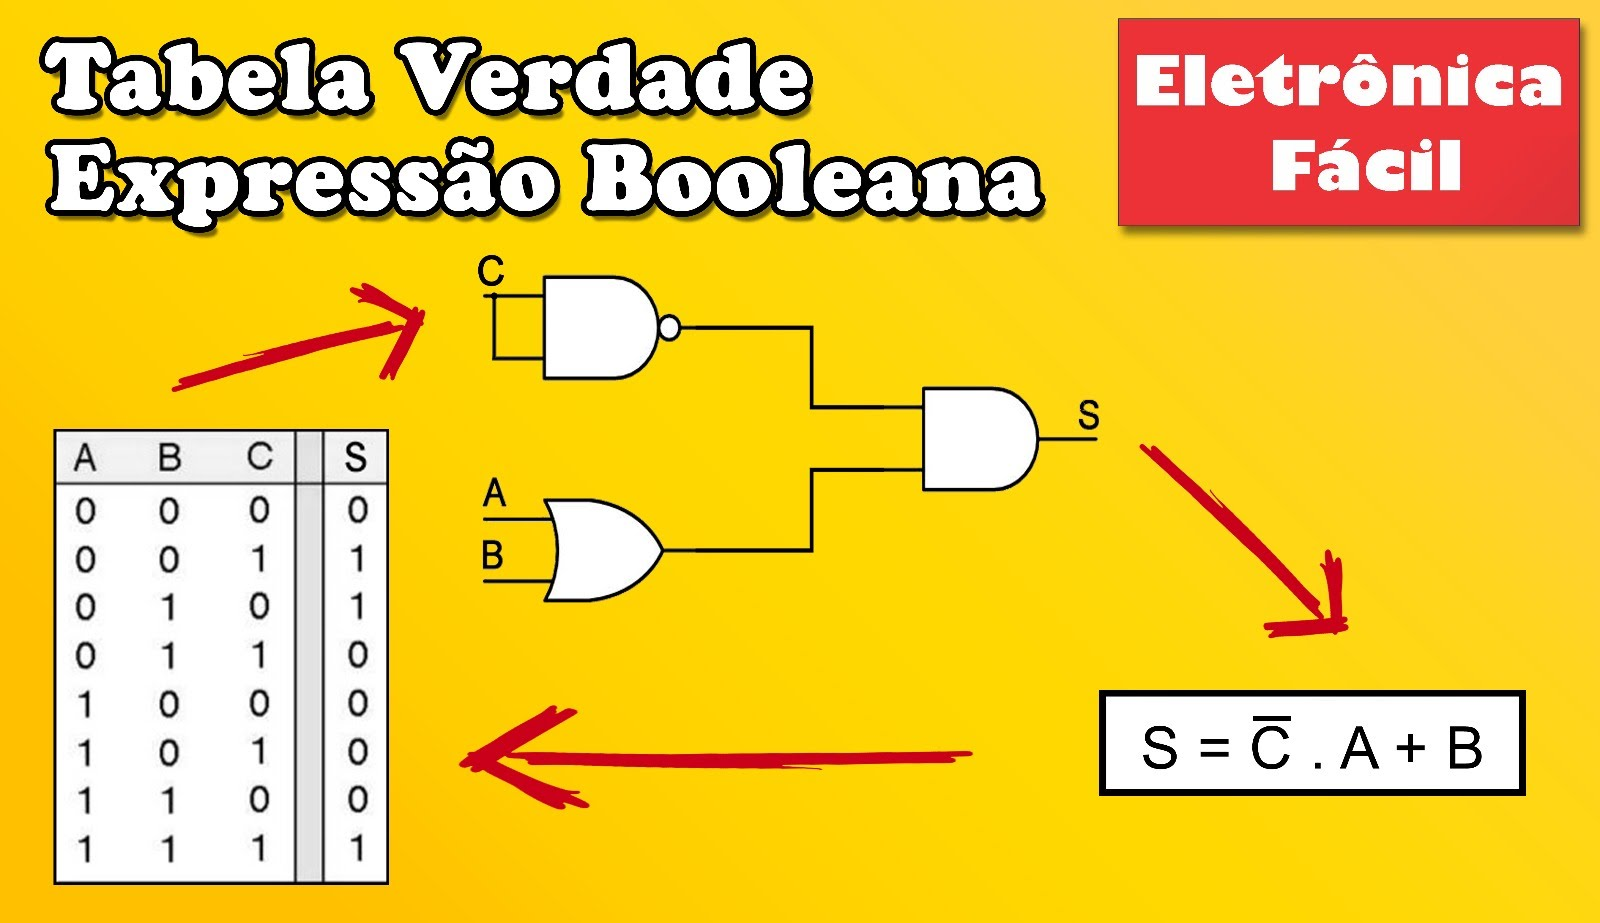
\includegraphics[width=0.75\linewidth]{Figuras/Ch4/conversao04.png}}
}

\frame{
	\frametitle{Como projetar um circuito digital?}
	\centering
	\begin{tikzpicture}[node distance=0.5cm, base/.style={
		% The shape:
		rectangle,minimum height=1cm,minimum width=1.5cm,rounded corners=3mm,align=center,
		% The rest
		very thick,draw=black!50,
		fill=black!20}]
	
		\node[base] (S) {Situação};
		\node[base,right=of S,text width=1.5cm] (TV) {Tabela verdade};
		\node[base, right=of TV, text width=2cm] (ES) {Expressão simplificada};
		\node[base, right=of ES] (C) {Circuito};
		
		\graph {(S) -> (TV) -> (ES) -> (C);};
		
	\end{tikzpicture}
%	\centerline{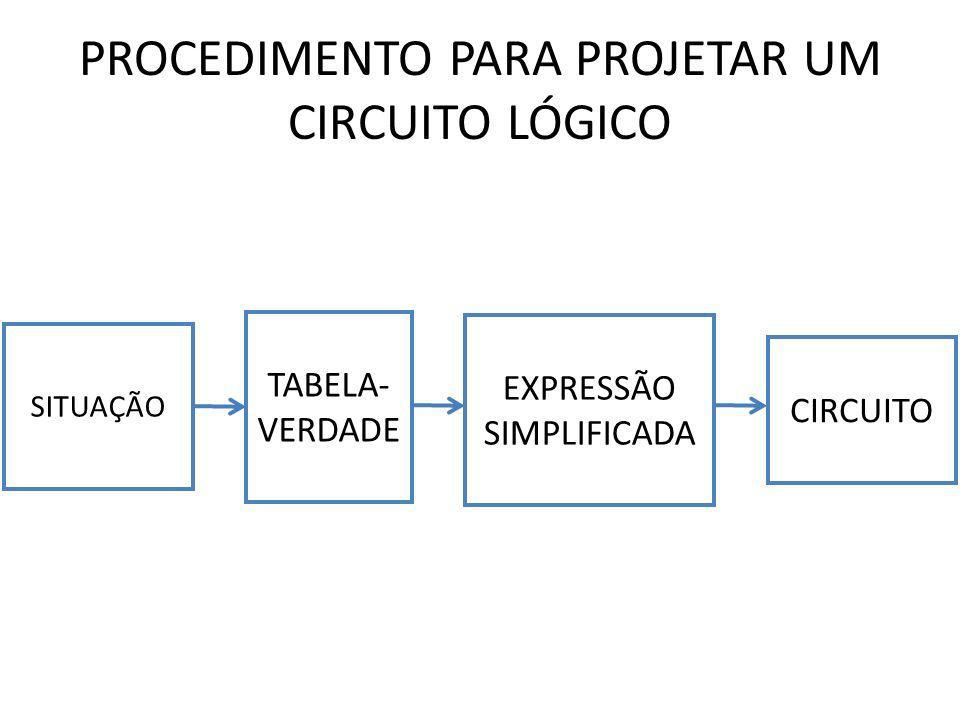
\includegraphics[width=0.75\linewidth]{Figuras/Ch4/resumo04.png}}
}

\frame{
	\frametitle{Resolução de projetos lógicos}
%	\centerline{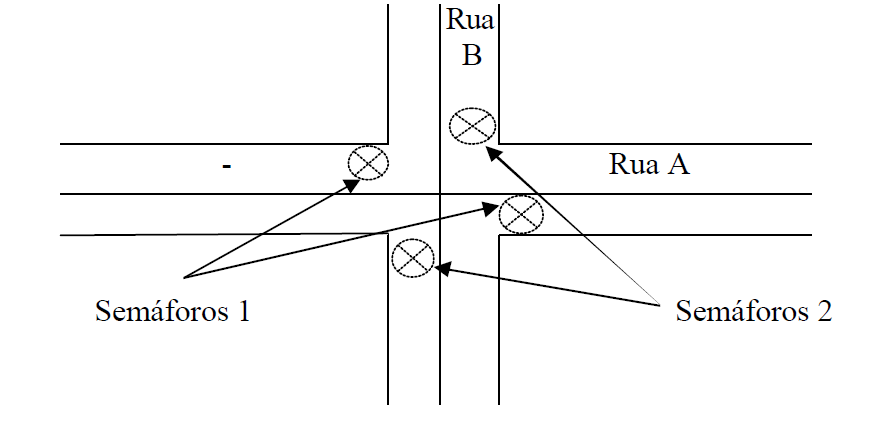
\includegraphics[width=0.75\linewidth]{Figuras/Ch4/2var.PNG}} 
	\begin{block}{Exemplo com duas variáveis}
		Caso tenha carro na(s)...
		\begin{itemize}
			\item Rua B
			\item Rua A
			\item Ruas A e B
		\end{itemize}
	\end{block}

	\centering
	\scalebox{0.9}{

\tikzset{every picture/.style={line width=0.75pt}} %set default line width to 0.75pt        

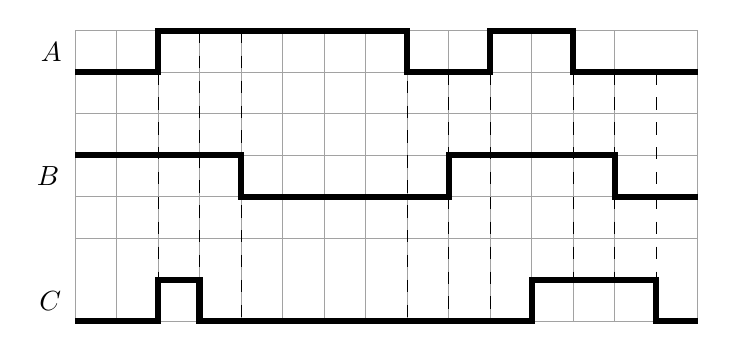
\begin{tikzpicture}[x=0.75pt,y=0.75pt,yscale=-1,xscale=1]
%uncomment if require: \path (0,300); %set diagram left start at 0, and has height of 300

%Shape: Grid [id:dp34531111101152123] 
\draw  [draw opacity=0] (100,40) -- (400,40) -- (400,180) -- (100,180) -- cycle ; \draw  [color={rgb, 255:red, 162; green, 162; blue, 162 }  ,draw opacity=1 ] (120,40) -- (120,180)(140,40) -- (140,180)(160,40) -- (160,180)(180,40) -- (180,180)(200,40) -- (200,180)(220,40) -- (220,180)(240,40) -- (240,180)(260,40) -- (260,180)(280,40) -- (280,180)(300,40) -- (300,180)(320,40) -- (320,180)(340,40) -- (340,180)(360,40) -- (360,180) ; \draw  [color={rgb, 255:red, 162; green, 162; blue, 162 }  ,draw opacity=1 ] (100,60) -- (400,60)(100,80) -- (400,80)(100,100) -- (400,100)(100,120) -- (400,120)(100,140) -- (400,140) ; \draw  [color={rgb, 255:red, 162; green, 162; blue, 162 }  ,draw opacity=1 ] (100,40) -- (400,40) -- (400,180) -- (100,180) -- cycle ;
%Straight Lines [id:da9908667716444586] 
\draw  [dash pattern={on 4.5pt off 4.5pt}]  (140,60) -- (140,160) ;


%Straight Lines [id:da9489034074703155] 
\draw  [dash pattern={on 4.5pt off 4.5pt}]  (160,40) -- (160,160) ;


%Straight Lines [id:da7444148673969375] 
\draw  [dash pattern={on 4.5pt off 4.5pt}]  (180,40) -- (180,180) ;


%Straight Lines [id:da33359589579811755] 
\draw  [dash pattern={on 4.5pt off 4.5pt}]  (260,40) -- (260,180) ;


%Straight Lines [id:da1689198722872045] 
\draw  [dash pattern={on 4.5pt off 4.5pt}]  (280,60) -- (280,180) ;


%Straight Lines [id:da2835936693187402] 
\draw  [dash pattern={on 4.5pt off 4.5pt}]  (300,60) -- (300,180) ;


%Straight Lines [id:da7069604701418795] 
\draw  [dash pattern={on 4.5pt off 4.5pt}]  (340,60) -- (340,160) ;


%Straight Lines [id:da35256438922338873] 
\draw  [dash pattern={on 4.5pt off 4.5pt}]  (360,60) -- (360,160) ;


%Straight Lines [id:da8396949759627998] 
\draw  [dash pattern={on 4.5pt off 4.5pt}]  (380,60) -- (380,160) ;


%Straight Lines [id:da8850959184881091] 
\draw [line width=2.25]    (100,60) -- (140,60) -- (140,40) -- (260,40) -- (260,60) -- (300,60) -- (300,40) -- (340,40) -- (340,60) -- (400,60) ;


%Straight Lines [id:da2574956876601695] 
\draw [line width=2.25]    (100,180) -- (140,180) -- (140,160) -- (160,160) -- (160,180) -- (320,180) -- (320,160) -- (380,160) -- (380,180) -- (400,180) ;


%Straight Lines [id:da8609754683162194] 
\draw [line width=2.25]    (100,100) -- (180,100) -- (180,120) -- (280,120) -- (280,100) -- (360,100) -- (360,120) -- (400,120) ;



% Text Node
\draw (88.5,50) node   {$A$};
% Text Node
\draw (87,110) node   {$B$};
% Text Node
\draw (88,170) node   {$C$};


\end{tikzpicture}
}
}

\frame{
	\frametitle{Resolução de projetos lógicos}
	
	\begin{block}{Exemplo com três variáveis}
		Conexão de 3 aparelhos a um amplificador, obedecendo às prioridades:
		\begin{itemize}
			\item CD player
			\item Tape playback
			\item Radio receptor
		\end{itemize}
	\end{block}

	\bigskip

	\centerline{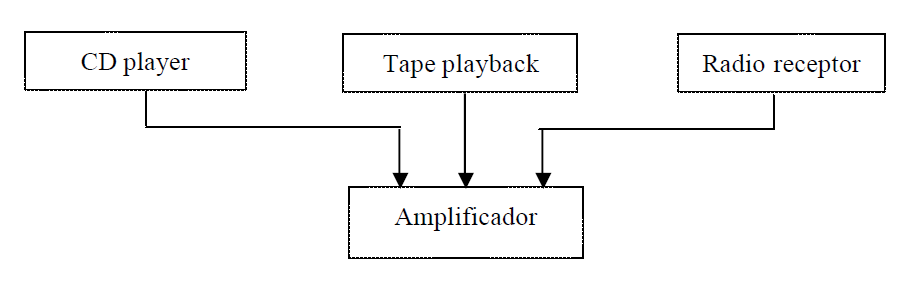
\includegraphics[width=1\linewidth]{Figuras/Ch4/3var.PNG}} 
}

\frame{
	\frametitle{Resolução de projetos lógicos}
	\begin{block}{Exemplo com quatro variáveis}
		Conexão de 4 setores, via intercomunicadores, a central da Secretária, obedecendo às prioridades:
		\begin{itemize}
			\item Presidente
			\item Vice Presidente
			\item Engenharia
			\item Chefes de Seção
		\end{itemize}
	\end{block}

	\centerline{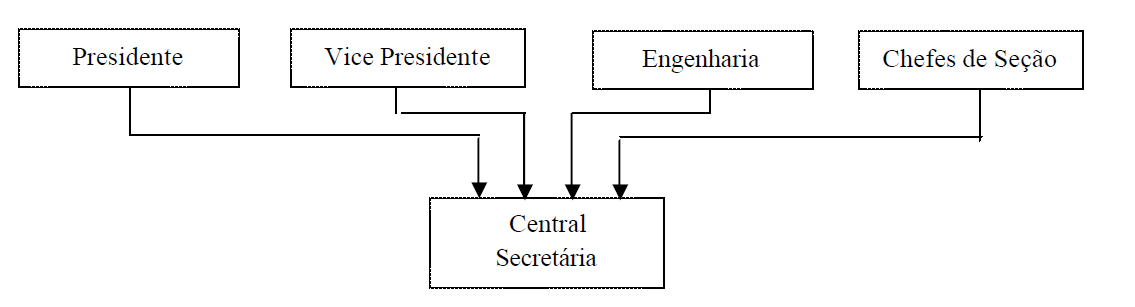
\includegraphics[width=1\linewidth]{Figuras/Ch4/4var.PNG}} 
}


\frame{
	\frametitle{Obtendo a expressão a partir do circuito - Exemplo \#01}
	\begin{center} \begin{circuitikz} \draw
			(0,2) node[and port] (myand) {}
			(2,1) node[or port] (myor) {}
			(myand.in 1) node[left=.5cm](a) {A}
			(myand.in 2) node[left =.5cm](b) {B}
			(myand.out) -| (myor.in 1)
			(a) -| (myand.in 1)
			(b) -| (myand.in 2)
			(b) node[below=1cm](c){C}
			(c) -| (myor.in 2)
			(myor.out) -- ++(.5cm,0) node[right] {S};
		\end{circuitikz} \end{center}
}

\frame{
	\frametitle{Obtendo a expressão a partir do circuito - Exemplo \#02}
	\begin{center} \begin{circuitikz}
			\draw
			(0,2) node[or port] (myor) {}
			(0,0) node[not port, scale=.5] (mynot) {}
			(2,1) node[nand port] (mynand) {}
			(myor.in 1) node[left=0.5cm](a) {A}
			(myor.in 2) node[left =.5cm](b) {B}
			(myor.out) -| (mynand.in 1)
			(a) -| (myor.in 1)
			(b) -| (myor.in 2);
			\node[coordinate] (p1) at ($ (myor.in 1)+(-0.5cm,0) $) {};
			\node[] (c) at (p1 |- mynot.in) {};
			\draw (mynot.in) -- (c) node[left] {C}
			(mynot.out) -| (mynand.in 2)
			(mynand.out) -- ++(.5cm,0) node[right] {S};
		\end{circuitikz} \end{center}
}

\frame{
	\frametitle{Obtendo a expressão a partir do circuito - Exemplo \#03}
	\begin{center} \begin{circuitikz} \draw
			(0,4) node[nor port] (mynor) {}
			(0,2) node[and port] (myand) {}
			(0,0) node[not port, scale=.5] (mynot) {}
			(2,3) node[nand port] (mynand) {}
			(4,1) node[or port] (myor) {}
			(mynor.in 1) node[left=.5cm](a) {A}
			(mynor.in 2) node[left =.5cm](b) {B}
			(mynor.out) -| (mynand.in 1)
			(myand.in 1) node[left=.5cm](c) {C}
			(myand.in 2) node[left =.5cm](d) {D}
			(myand.out) -| (mynand.in 2);
			\node[coordinate] (p1) at ($ (mynor.in 1)+(-0.5cm,0) $) {};
			\node[] (e) at (p1 |- mynot.in) {};
			\draw (a) -| (mynor.in 1)
			(b) -| (mynor.in 2)
			(c) -| (myand.in 1)
			(d) -| (myand.in 2)
			(mynot.in) -- (e) node[left] {E}
			(mynand.out) -| (myor.in 1)
			(mynot.out) -| (myor.in 2)
			(myor.out) -- ++(.5cm,0) node[right] {S};
		\end{circuitikz} \end{center}
}


\frame{
	\frametitle{Obtendo o circuito a partir da expressão}
	\begin{block}{Hierarquia}
		\begin{itemize}
			\item Parênteses.
			\item Bloco AND.
			\item Bloco OR.
			\item Negação.
		\end{itemize}
	\end{block}
}

\frame{
	\frametitle{Obtendo o circuito a partir da expressão}
	\begin{block}{Exercícios}
		\begin{itemize}
			\item $S = (A + B)\cdot C\cdot (B+D)$
			\item $Z = (\notted{A\cdot B} \oplus A) + (\notted{A} + B)$
			\item $Y = (A\cdot B) + \notted{C}\cdot D$
			\item $X = (A + B + C)\cdot \notted{(\notted{A} + C)\cdot (A + \notted{B})}$
		\end{itemize}
	\end{block}
}

\frame{
	\frametitle{Obtendo a tabela verdade a partir da expressão}
	\begin{block}{Tabela verdade}
		A \textbf{tabela verdade} deve registrar \textbf{todas as possibilidades} de um dada expressão booleana, e pode ser obtida através dos seguintes passos:
		\begin{enumerate}
			\item Monte o quadro de possibilidades.
			\item \textbf{n} colunas para as variáveis.
			\item Use colunas auxiliares para os membros.
			\item Monte uma coluna para o resultado final.
		\end{enumerate}
	\end{block}
}

\frame{
	\frametitle{Obtendo a tabela verdade a partir da expressão}
	\begin{block}{Exemplo \#01}
		\[ Z = (\notted{A\cdot B} \oplus A) + (\notted{A} + B) \]
		
		\bigskip
		\centering
%		\renewcommand{\arraystretch}{1}
		\resizebox{1\textwidth}{!}{
		\begin{tabular}{cc|c|c|c|c|c}
			\toprule
			$ A $ & $ B $ & $\notted{A\cdot B} $ & $\notted{A\cdot B} \oplus A$ & $\notted{A}$ & $\notted{A} + B$ & \textcolor{green}{S} \\ \midrule
			0 & 0 & 1 &	\textcolor{red}1 & 1 & \textcolor{red}1 & \textcolor{blue}1 \\
			0 & 1 & 1 & \textcolor{red}1 & 1 & \textcolor{red}1 & \textcolor{blue}1 \\
			1 & 0 & 1 & \textcolor{red}0 & 0 & \textcolor{red}0 & \textcolor{blue}0 \\
			1 & 1 & 0 & \textcolor{red}1 & 0 & \textcolor{red}1 & \textcolor{blue}1 \\  \bottomrule
	\end{tabular}}
	\end{block}
}

\frame{
	\frametitle{Obtendo a tabela verdade a partir da expressão}
	\begin{block}{Exercícios}
		\begin{itemize}
			\item $S = (A\cdot \notted{B}\cdot C) + (A\cdot \notted{D}) + (\notted{A}\cdot B\cdot D)$
			\item $Z = \notted{A} + B + A\cdot \notted{B}\cdot \notted{C}$
			\item $Y = C \oplus (\notted{A.B})$
			\item $X = A\cdot \notted{B} + \notted{A}\cdot B$
		\end{itemize}
	\end{block}
}

\frame{
	\frametitle{Obtendo a expressão a partir da tabela verdade}
	\begin{block}{Situação mais utilizada}
		\textbf{Lembre-se do problema inicial}
		\begin{itemize}
			\item Situação.
			\item Tabela verdade.
			\item Expressão booleana.
			\item Circuito lógico.
		\end{itemize}
			
			\bigskip
			
			\textbf{MINTERMOS}: saídas iguais a \textbf{1} - \textcolor{red}{SoP}
			
			\bigskip
			
			\textbf{MAXTERMOS}: saídas iguais a \textbf{0} - \textcolor{red}{PoS}
	\end{block}
}

\frame{
	\frametitle{Obtendo a expressão a partir da tabela verdade}
	\begin{block}{MINTERMOS}
		\begin{itemize}
			\item Saídas iguais a \textbf{1} - \textcolor{red}{SoP}
		\end{itemize}
	\end{block}

	\renewcommand{\arraystretch}{1}
	\centering
	\begin{tabular}{ccc|c}
		\toprule
		A & B & C & S                \\ \midrule
		0 & 0 & 0 & \textcolor{red}1 \\
		0 & 0 & 1 & \textcolor{red}1 \\
		0 & 1 & 0 & \textcolor{red}1 \\
		0 & 1 & 1 & 0                \\
		1 & 0 & 0 & 0                \\
		1 & 0 & 1 & \textcolor{red}1 \\
		1 & 1 & 0 & 0                \\
		1 & 1 & 1 & \textcolor{red}1 \\ \bottomrule
	\end{tabular}

	\begin{block}{Expressão final}
		\vspace{-0.3cm}
		\[ S = (\notted{A} \cdot \notted{B}\cdot \notted{C}) + (\notted{A} \cdot \notted{B}\cdot C) + (\notted{A}\cdot B\cdot \notted{C}) + (A\cdot \notted{B}\cdot C) + (A\cdot B\cdot C) \]
	\end{block}

}

\frame{
	\frametitle{Obtendo a expressão a partir da tabela verdade}
	\begin{block}{MAXTERMOS}
		\begin{itemize}
			\item Saídas iguais a \textbf{0} - \textcolor{red}{PoS}
		\end{itemize}
	\end{block}

	\renewcommand{\arraystretch}{1}
	\centering
	\begin{tabular}{ccc|c}
		\toprule
		A & B & C & S                        \\ \midrule
		0 & 0 & 0 & 1                        \\
		0 & 0 & 1 & 1                        \\
		0 & 1 & 0 & 1                        \\
		0 & 1 & 1 & \textcolor{red}0         \\
		1 & 0 & 0 & \textcolor{red}0         \\
		1 & 0 & 1 & 1                        \\
		1 & 1 & 0 & \textcolor{red} 0        \\ 
		1 & 1 & 1 & 1                        \\ \bottomrule
	\end{tabular}

	\begin{block}{Expressão final}
		\vspace{-0.15cm}
		\[ S = (A + \notted{B} + \notted{C})\cdot (\notted{A}  + B + C)\cdot (\notted{A} + \notted{B} + C) \]
	\end{block}
}


\section*{Exercícios}
\frame{
	\frametitle{Exercícios}
	\begin{block}{}
		01. A partir da tabela verdade abaixo encontre a expressão booleana por mintermos e maxtermos. Após isto, implemente ambos os circuitos digitais.
	\end{block}

	\medskip

	\renewcommand{\arraystretch}{1}
	\centering
	\begin{tabular}{ccc|c}
		\toprule
		A & B & C & S \\ \midrule
		0 & 0 & 0 & 0 \\
		0 & 0 & 1 & 1 \\
		0 & 1 & 0 & 1 \\
		0 & 1 & 1 & 0 \\
		1 & 0 & 0 & 1 \\
		1 & 0 & 1 & 0 \\
		1 & 1 & 0 & 0 \\
		1 & 1 & 1 & 1 \\ \bottomrule
	\end{tabular}
}

\section*{Referências}


\frame{
	\frametitle{Referências e exercícios complementares}
	\begin{itemize}
		\item IDOETA, Ivan V. e CAPUANO, Francisco G. Elementos de Eletrônica Digital. São Paulo:
		      Editora Érica, ed. 40. 2008.
	\end{itemize}

	\centering{\alert{Página 82 - \textbf{2.9.2 até 2.9.13, 2.9.15 até 2.9.17}}}

}